\documentclass[12pt]{article}

%useful packages
\usepackage{color,soul}
\usepackage[usenames,dvipsnames,svgnames,table]{xcolor}
\usepackage{amsmath,amsthm,amscd,amssymb,bm}
\usepackage{hyperref}
\hypersetup{
    colorlinks=true,
    linkcolor=JungleGreen
}
\usepackage[utf8]{inputenc}
\usepackage[top=2cm, bottom=3cm, left=2cm, right=2cm]{geometry}
\usepackage{pgfplots}
\usepackage{enumitem}
\usepgfplotslibrary{fillbetween}
\usetikzlibrary{patterns}
\usepackage{tcolorbox}
\usepackage{centernot}
\usepackage{mathtools}
\usepackage{xcolor}

% Packages to create table 1
\usepackage{pdflscape}
\usepackage{subfig}
\usepackage{graphicx}


%personal definitions and commands
\newcommand{\R}{\mathbb{R}} 
\newcommand{\E}{\mathbb{E}}
\newcommand{\V}{\mathbb{V}}
\newcommand{\C}{\mathbb{C}}
\newcommand{\Prob}{\mathbb{P}}
\newcommand{\e}{\epsilon}
\newcommand\numberthis{\addtocounter{equation}{1}\tag{\theequation}} %allows numbering of single equations in align* environment
\newcommand{\mtx}[1]{\ensuremath{\bm{\mathit{#1}}}}
\newcommand{\B}{\hat{\boldsymbol{\beta}}}
\newcommand{\Cov}{\mathbb{C}\text{ov}}
\newcommand{\N}{\mathcal{N}}



\title{ECON675 -- Assignment 4}
\author{Anirudh Yadav}
\setlength\parindent{0pt}
\begin{document}

\maketitle

\setcounter{tocdepth}{2}
\tableofcontents

\newpage

\section{Estimating equations}

\subsection{Moment conditions}
The goal of this question is to show that the four given functions are valid moment conditions for the parameter $\theta_t(g)$. That is, we want to show that 
\begin{align*}
\E[\psi_{\texttt{f},t}(\mtx{Z}_i; \theta_t(g))] = 0,
\end{align*}
for each $\texttt{f} \in \{\texttt{IPW},\texttt{RI1},\texttt{RI2}, \texttt{DR}\}$. Note that in the derivations below I invoke LIE a lot without specifically mentioning it.\\

Start with the inverse probability weighting function
\begin{align*}
\E[\psi_{\texttt{IPW},t}(\mtx{Z}_i; \theta_t(g))] &=\E\left[\frac{D_i(t)\cdot g(Y_i(t))}{p_t(\mtx{X}_i)}\right] - \theta_t(g)\\
&=\E\left[\E\left[\frac{D_i(t)\cdot g(Y_i(t))}{p_t(\mtx{X}_i)}| \mtx{X}_i\right]\right] - \theta_t(g)\\
&=\E\left[\frac{1}{p_t(\mtx{X}_i)}\E\left[D_i(t)|\mtx{X}_i\right]\E\left[ g(Y_i(t))| \mtx{X}_i\right]\right] - \theta_t(g)
\end{align*}
Now, 
\begin{align*}
\E\left[D_i(t)|\mtx{X}_i\right] & = \Pr[D_i(t)=1|\mtx{X}_i] = \Pr[T_i = t|\mtx{X}_i] = p_t(\mtx{X}_i).
\end{align*}
Thus,
\begin{align*}
\E[\psi_{\texttt{IPW},t}(\mtx{Z}_i; \theta_t(g))] &= \E\left[\E\left[ g(Y_i(t))| \mtx{X}_i\right]\right] - \theta_t(g)\\
&=\E[g(Y_i(t))] - \theta_t(g)\\
&=0.
\end{align*}
Next, consider
\begin{align*}
\E[\psi_{\texttt{RI1},t}(\mtx{Z}_i; \theta_t(g))] &= \E[e_t(g;\mtx{X}_i)] - \theta_t(g)\\
&=\E[\E[g(Y_i(t)|\mtx{X}_i]] - \theta_t(g)\\
&=\E[g(Y_i(t)] -  \theta_t(g)\\
&=0.
\end{align*}
And,
\begin{align*}
\E[\psi_{\texttt{RI2},t}(\mtx{Z}_i; \theta_t(g))] &= \E\left[\frac{D_i(t)\cdot e_t(g;\mtx{X}_i)}{p_t(\mtx{X}_i)}\right]  - \theta_t(g)\\
&=\E\left[\E\left[\frac{D_i(t)\cdot e_t(g;\mtx{X}_i)}{p_t(\mtx{X}_i)}| \mtx{X}_i\right]\right] - \theta_t(g)\\
&=\E\left[\E\left[e_t(g;\mtx{X}_i)| \mtx{X}_i\right]\right] - \theta_t(g)\\
&= \E[e_t(g;\mtx{X}_i)] - \theta_t(g)\\
&=0.
\end{align*}
Finally, consider the doubly robust function
\begin{align*}
\E[\psi_{\texttt{DR},t}(\mtx{Z}_i; \theta_t(g))] &= \E\left[\frac{D_i(t)\cdot g(Y_i(t))}{p_t(\mtx{X}_i)}\right] - \theta_t(g) - \E\left[\frac{e_t(g;\mtx{X}_i)}{p_t(\mtx{X}_i)}(D_i(t)-p_t(\mtx{X}_i))\right].
\end{align*}
Using the IPW result above, we know that the first two terms cancel each other out, so that
\begin{align*}
\E[\psi_{\texttt{DR},t}(\mtx{Z}_i; \theta_t(g))] &=- \E\left[\frac{e_t(g;\mtx{X}_i)}{p_t(\mtx{X}_i)}(D_i(t)-p_t(\mtx{X}_i))\right]\\
&=- \E\left[\frac{e_t(g;\mtx{X}_i)D_i(t)}{p_t(\mtx{X}_i)}\right] + \E[e_t(g;\mtx{X}_i)]\\
&= -\theta_t(g) + \theta_t(g)\\
&=0.
\end{align*}
So each of the four functions is a valid moment condition for $\theta_t(g)$.

\subsection{Plug-in estimators}
The plug-in IPW estimator is 
\begin{align*}
\hat{\theta}_{\texttt{IPW},t}(g) = \frac{1}{n}\sum_{i=1}^n\frac{D_i(t)g(Y_i)}{\hat p_t(\mtx{X}_i)},
\end{align*}
where $\hat p_t(\mtx{X}_i)$ is the estimated propensity score. Note that since there are multiple treatment levels, the estimated propensity score would have to be computed using a suitable discrete choice model. For instance, $\hat p_t(\mtx{X}_i)$ could be estimated using a multinomial logit model.\\

The plug-in projection (or regression imputation) estimator is
\begin{align*}
\hat{\theta}_{\texttt{RI1},t}(g) = \hat{\E}[e_t(g;\mtx{X}_i)] =  \frac{1}{n}\sum_{i=1}^n \hat{\E}[g(Y_i(t))|\mtx{X}_i] &=  \frac{1}{n}\sum_{i=1}^n \hat{\E}[g(Y_i(t))|\mtx{X}_i, D_i(t)=1] \\
&= \frac{1}{n}\sum_{i=1}^n \hat{\E}[g(Y_i)|\mtx{X}_i, D_i(t)=1],
\end{align*}
where the second last equality uses the ignorability assumption. We need to make a choice about how to estimate the conditional expectation term. I think we could use NLS, or possibly a nonparametric method like kernel regression. To ease notation, let $\widehat{\mu}_t(\mtx{X}_i)$ be the parametric or nonparametric estimate of $\E[g(Y_i)|\mtx{X}_i, D_i(t)=1]$. Then, the projection estimator is
\begin{align*}
\hat{\theta}_{\texttt{RI1},t}(g) = \frac{1}{n}\sum_{i=1}^n \widehat{\mu}_t(\mtx{X}_i)
\end{align*}

The plug-in `hybrid' imputation estimator
\begin{align*}
\hat{\theta}_{\texttt{RI2},t}(g) &=  \frac{1}{n}\sum_{i=1}^n\frac{D_i(t)\widehat{\mu}_t(\mtx{X}_i)}{\hat p_t(\mtx{X}_i)}. 
\end{align*}
Finally, the plug-in doubly robust estimator is given by
\begin{align*}
\hat{\theta}_{\texttt{DR},t}(g) &= \frac{1}{n}\sum_{i=1}^n\frac{D_i(t)g(Y_i)}{\hat p_t(\mtx{X}_i)}-\frac{1}{n}\sum_{i=1}^n\frac{\widehat{\mu}_t(\mtx{X}_i)}{\hat p_t(\mtx{X}_i)}(D_i(t) - \hat p_t(\mtx{X}_i))\\
&=\frac{1}{n}\sum_{i=1}^n \left(\frac{D_i(t)(g(Y_i) - \widehat{\mu}_t(\mtx{X}_i))}{\hat p_t(\mtx{X}_i)} + \widehat{\mu}_t(\mtx{X}_i) \right).
\end{align*}
As discussed in Abadie and Catteneo (2018), the relative performance of the above estimators depends on the features of the data generating process. In finite samples, IPW estimators become unstable when the propensity score approaches zero or one and regression imputation estimators may suffer from extrapolation biases. Doubly robust estimators include safeguards against bias caused by misspecification but impose additional specification choices that may affect the resulting estimate.

\subsection{Estimating the variance of potential outcomes}
Note that 
\begin{align*}
\sigma_t^2 = \V[Y_i(t)] = \E\left[Y_i(t) - \E[Y_i(t)]\right]^2
\end{align*}
Thus, we can estimate $\sigma_t^2$ using any of the above methods, with $g(Y_i(t)) = \E\left[Y_i(t) - \E[Y_i(t)]\right]^2$. Note that this is a two-step estimator, since it requires an estimate of $\E[Y_i(t)]$. To conduct the hypothesis test of $H_0: \sigma_t^2 = \sigma^2 \text{ } \forall t \in \mathcal{T}$ we would need to use an appropriate joint hypothesis testing procedure. One way to proceed would be test  $H_0: \sigma_t^2 - \sigma^2 =0 \text{ } \forall t \in \mathcal{T}$  and construct the vector $\widehat{\mtx{\theta}}= (\hat \sigma^2_1-\sigma^2,...,\hat\sigma^2_T-\sigma^2)'$, and then show $\sqrt{n}(\widehat{\mtx{\theta}}-\mtx{\theta}_0) \to \N(0,V)$. Then, the Delta method implies $\sqrt{n}(||\widehat{\mtx{\theta}}||^2-||\mtx{\theta}_0||^2) \to \N(0,4\mtx{\theta}_0'V\mtx{\theta}_0)$. Note that under the null $\mtx{\theta}_0=0$, so we can now conduct the hypothesis test $H_0: \mtx{\theta}_0=0$ in the usual way, using an estimator for the asymptotic variance.


\newpage
\section{Estimating average treatment effects}

Estimation results are overleaf. Estimates of ATEs are very different across the Lalonde and PSID control samples (for all estimators), which suggests that there are large and systematic differences between the two control groups . For instance, ATEs are generally positive when using the Lalonde control, while many ATEs are large and negative when using the PSID control group. This makes sense because the NSW program was targeted at individuals who had faced economic and social problems prior to enrolment (i.e. these respondents, on average, had low incomes), whereas the PSID sample is more representative of the entire US population. \\

Most estimates of ATTs are broadly similar across the samples. The ATTs using matching estimators are quite similar across both samples. Again, this makes sense, because matching estimators specifically ensure that there is a decent degree of covariate balance between the treatment and control samples (i.e. the matching estimators would pick respondents from the PSID sample who have similar characteristics to the respondents in the Lalonde experiment).\\

I had some issues with the estimation of both ATEs and ATTs:
\begin{itemize}
\item I had problem getting RI/IPW/DR estimates for PSID covariate set A in \verb|R| (using the \verb|CausalGAM| package) so I used \verb|STATA| only in this case.
\item IPW and DR ATT estimates are the same in \verb|STATA|; I'm not sure why.
\item Many of the logit regressions for estimating propensity scores did not converge, so I generally set the maximum number of iterations to 25.
\end{itemize}



\begin{landscape}
\begin{table}
\centering
\caption{Estimation and Inference on ATE and ATT}\label{tab:tableQ2}
\vspace{-.1in}\resizebox{\columnwidth}{!}{
\subfloat[][ATE]{\input{teffectsATEq.txt}}\quad
\subfloat[][ATT]{\input{teffectsATTq.txt}}
}
\end{table}
\end{landscape}

\newpage

\section{Post-model selection inference}

\subsection{Summary statistics and density plots}
The summary statistics for each estimator are presented in Table 2 and the kernel density plots (using an Epanechnikov kernel and \verb|R|'s unbiased cross-validated bandwidth) are just below. As expected, the empirical distribution of $\hat{\beta}$ is approximately normal with a mean very close to the true parameter, $\beta_0=0.5$. The empirical distribution of $\tilde{\beta}$ looks fairly normal, but clearly $\tilde{\beta}$ is inconsistent for $\beta_0$. As expected, the empirical distribution of $\check{\beta}$ is clearly not normal, and the mean is a bit than the true parameter.

\begin{table}[!htpb]
\centering
\caption{\textbf{Summary Statistics for each Estimator}}
\begin{tabular}{crrrrrr}
  \hline
Estimator & Min. & 1st Qu. & Median & Mean & 3rd Qu. & Max. \\ 
  \hline
(i) $\hat{\beta}$ & -0.50 & 0.32 & 0.52 & 0.51 & 0.71 & 1.32 \\ 
(ii) $\tilde{\beta}$ & 0.77 & 1.26 & 1.36 & 1.36 & 1.47 & 1.88 \\ 
(iii) $ \check{\beta}$& -0.50 & 0.32 & 0.52 & 0.54 & 0.72 & 1.66 \\ 
   \hline
\end{tabular}
\end{table}

\begin{figure}[!htpb]
    \centering
    
        %\centering
        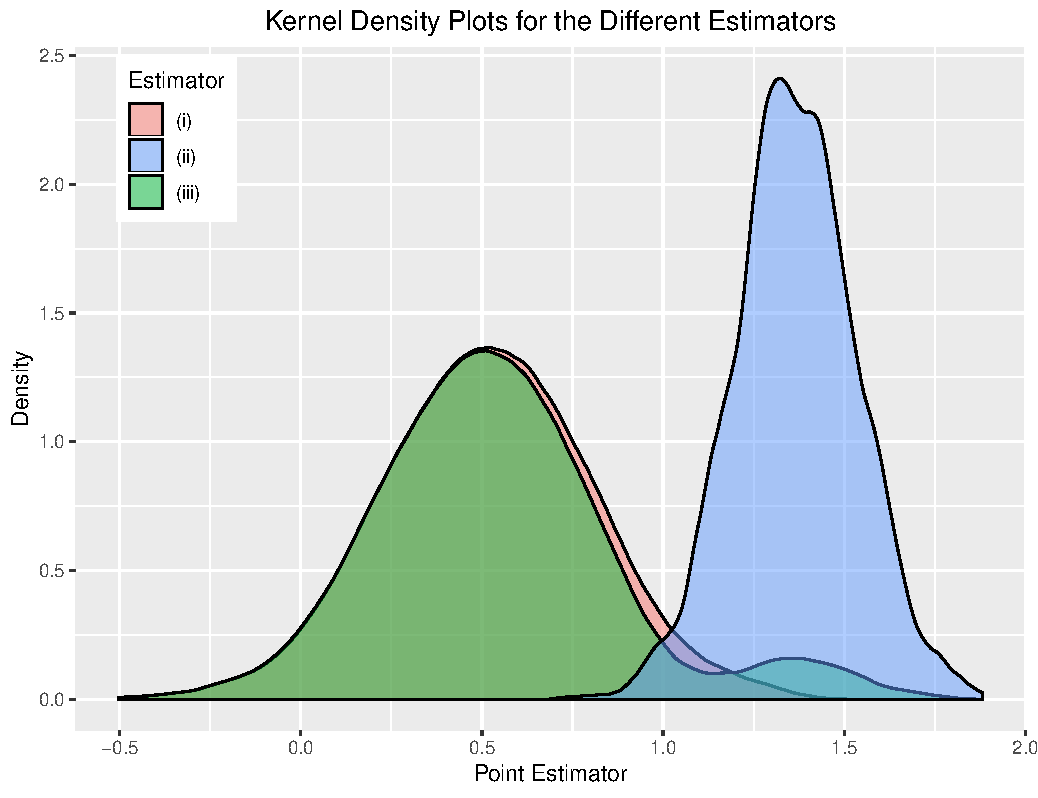
\includegraphics[width=0.7\textwidth]{dens.pdf}

\end{figure}

\subsection{Coverage rates}
To compute the coverage rates, I first create an indicator variable which is equal to 1 if, for a given simulation, the 95\% asymptotic CI contains the true parameter $\beta_0 = 0.5$; I do this for each estimator and then take the mean of the indicator variable to get the coverage rate. Note that the asymptotic CI using $\check{\beta}$ is just equal to the CI using $\hat{\beta}$ whenever $\check{\beta}=\hat{\beta}$, and equal to the CI using $\tilde{\beta}$ otherwise.\\

The $\hat{\beta}$'s coverage rate is 0.936, which is very close to 0.95, as expected. In contrast, $\tilde{\beta}$'s coverage rate is only 0.001, which is unsurprising since $\tilde{\beta}$ is inconsistent for $\beta_0$. Finally, $\check{\beta}$'s coverage rate is 0.900, which is because $\check{\beta}$ is also inconsistent for $\beta_0$.

\newpage

\section{Appendix}

\subsection{\texttt{R} code}

\subsubsection{Question 2}
\scriptsize
\begin{verbatim}
## ECON675: ASSIGNMENT 4
## Q2: ESTIMATING AVERAGE TREATMENT EFFECTS
## Anirudh Yadav 
## 11/06/2018

######################################################################
# Load packages, clear workspace
######################################################################
rm(list = ls())             #clear workspace
library(foreach)            #for looping
library(data.table)         #for data manipulation
library(Matrix)             #fast matrix calcs
library(ggplot2)            #for pretty plots
library(sandwich)           #for variance-covariance estimation 
library(xtable)             #for latex tables
library(boot)               #for bootstrapping
library(CausalGAM)          #for computing ATEs
options(scipen = 999)       #forces R to use normal numbers instead of scientific notation

######################################################################
# Input data, add covariates and subset data
######################################################################
data <- as.data.table(read.csv('PhD_Coursework/ECON675/HW4/LaLonde_all.csv'))

data = data[,log.re74:=log(re74+1)]
data = data[,log.re75:=log(re75+1)]
data = data[,age.sq:=age^2]
data = data[,educ.sq:=educ^2]
data = data[,age.cu:=age^3]
data = data[,black.u74:=black*u74]
data = data[,educ.logre74:=educ*log.re74]

# subset data for LaLonde control only
X.ll = data[treat==1 | treat==0]
Y.ll = data[treat==1 | treat==0,.(re78)]

# subset data for PSID control only
X.ps = data[treat==1 | treat==2]
Y.ps = data[treat==1 | treat==2,.(re78)]

# Recode treatment indicate in PSID control dataset (recode 2's as 0's)
X.ps = X.ps[,treat:=as.numeric(treat==1)]


######################################################################
# Create covariate sets
######################################################################
X.ll.0  = X.ll[,.(treat)]
X.ps.0  = X.ps[,.(treat)]

X.ll.A  = X.ll[,-c("age.sq","educ.sq","age.cu","black.u74","educ.logre74","u74","u75","re78","re74","re75")]
X.ps.A  = X.ps[,-c("age.sq","educ.sq","age.cu","black.u74","educ.logre74","u74","u75","re78","re74","re75")]

X.ll.B  =  X.ll[,-c("age.cu","black.u74","educ.logre74","re78","re74","re75")]
X.ps.B  =  X.ps[,-c("age.cu","black.u74","educ.logre74","re78","re74","re75")]

X.ll.C  =  X.ll[,-c("re78","re74","re75")]
X.ps.C  =  X.ps[,-c("re78","re74","re75")]

######################################################################
# [1] Difference in means
######################################################################
dmeans.ll = lm(as.matrix(Y.ll)~as.matrix(X.ll.0))
dmeans.ps = lm(as.matrix(Y.ps)~as.matrix(X.ps.0))

# Compute robust standard errors
dmeans.ll.se    = sqrt(diag(vcovHC(dmeans.ll, type = "HC1")))
dmeans.ps.se    = sqrt(diag(vcovHC(dmeans.ps, type = "HC1")))

# Compute 95% CIs
dmeans.ll.lower = dmeans.ll$coefficients - 1.96*dmeans.ll.se
dmeans.ll.upper = dmeans.ll$coefficients + 1.96*dmeans.ll.se

dmeans.ps.lower = dmeans.ps$coefficients - 1.96*dmeans.ps.se
dmeans.ps.upper = dmeans.ps$coefficients + 1.96*dmeans.ps.se

# Put results together
dmeans.ll.results = cbind(dmeans.ll$coefficients,dmeans.ll.se,dmeans.ll.lower,dmeans.ll.upper)
dmeans.ps.results = cbind(dmeans.ps$coefficients,dmeans.ps.se,dmeans.ps.lower,dmeans.ps.upper)


######################################################################
# [2] OLS
######################################################################
# Compute OLS coefficients
ols.ll.A = lm(as.matrix(Y.ll)~as.matrix(X.ll.A))
ols.ps.A = lm(as.matrix(Y.ps)~as.matrix(X.ps.A))
ols.ll.B = lm(as.matrix(Y.ll)~as.matrix(X.ll.B))
ols.ps.B = lm(as.matrix(Y.ps)~as.matrix(X.ps.B))
ols.ll.C = lm(as.matrix(Y.ll)~as.matrix(X.ll.C))
ols.ps.C = lm(as.matrix(Y.ps)~as.matrix(X.ps.C))

# Compute robust standard errors
ols.ll.se.A    = sqrt(diag(vcovHC(ols.ll.A, type = "HC1")))
ols.ps.se.A    = sqrt(diag(vcovHC(ols.ps.A, type = "HC1")))
ols.ll.se.B    = sqrt(diag(vcovHC(ols.ll.B, type = "HC1")))
ols.ps.se.B    = sqrt(diag(vcovHC(ols.ps.B, type = "HC1")))
ols.ll.se.C    = sqrt(diag(vcovHC(ols.ll.C, type = "HC1")))
ols.ps.se.C    = sqrt(diag(vcovHC(ols.ps.C, type = "HC1")))

# Compute 95% CIs
ols.ll.lower.A = ols.ll.A$coefficients - 1.96*ols.ll.se.A
ols.ll.upper.A = ols.ll.A$coefficients + 1.96*ols.ll.se.A
ols.ps.lower.A = ols.ps.A$coefficients - 1.96*ols.ps.se.A
ols.ps.upper.A = ols.ps.A$coefficients + 1.96*ols.ps.se.A
ols.ll.lower.B = ols.ll.B$coefficients - 1.96*ols.ll.se.B
ols.ll.upper.B = ols.ll.B$coefficients + 1.96*ols.ll.se.B
ols.ps.lower.B = ols.ps.B$coefficients - 1.96*ols.ps.se.B
ols.ps.upper.B = ols.ps.B$coefficients + 1.96*ols.ps.se.B
ols.ll.lower.C = ols.ll.C$coefficients - 1.96*ols.ll.se.C
ols.ll.upper.C = ols.ll.C$coefficients + 1.96*ols.ll.se.C
ols.ps.lower.C = ols.ps.C$coefficients - 1.96*ols.ps.se.C
ols.ps.upper.C = ols.ps.C$coefficients + 1.96*ols.ps.se.C

# Put treatment effect results together 
ols.ll.results = cbind(c(ols.ll.A$coefficients[2],ols.ll.B$coefficients[2],ols.ll.C$coefficients[2]),c(ols.ll.se.A[2],ols.ll.se.B[2],ols.ll.se.C[2]),c(ols.ll.lower.A[2],ols.ll.lower.B[2],ols.ll.lower.C[2]),c(ols.ll.upper.A[2],ols.ll.upper.B[2],ols.ll.upper.C[2]))
ols.ps.results = cbind(c(ols.ps.A$coefficients[2],ols.ps.B$coefficients[2],ols.ps.C$coefficients[2]),c(ols.ps.se.A[2],ols.ps.se.B[2],ols.ps.se.C[2]),c(ols.ps.lower.A[2],ols.ps.lower.B[2],ols.ps.lower.C[2]),c(ols.ps.upper.A[2],ols.ps.upper.B[2],ols.ps.upper.C[2]))


######################################################################
# [3.A] Regression Imputation, covariate set A
######################################################################

# Subset outcome data for imputation
Y.treat        = data[treat==1,.(re78)]
Y.control.ll   = data[treat==0,.(re78)]
Y.control.ps   = data[treat==2,.(re78)]

# Subset covariates for imputation
X.treat.A       = data[treat==1,-c("age.sq","educ.sq","age.cu","black.u74","educ.logre74","u74","u75","re78","re74","re75","treat")]
X.control.ll.A  = data[treat==0,-c("age.sq","educ.sq","age.cu","black.u74","educ.logre74","u74","u75","re78","re74","re75","treat")]
X.control.ps.A  = data[treat==2,-c("age.sq","educ.sq","age.cu","black.u74","educ.logre74","u74","u75","re78","re74","re75","treat")]

# Get OLS coefficients for imputation
ols.treat.A          = lm(as.matrix(Y.treat)~as.matrix(X.treat.A))
ols.control.ll.A     = lm(as.matrix(Y.control.ll)~as.matrix(X.control.ll.A))
ols.control.ps.A     = lm(as.matrix(Y.control.ps)~as.matrix(X.control.ps.A))

# I need to add constants to the X's to compute imputed treatment effects,
# Then reorder so const is the first variable
X.treat.A[,const:=1]
setcolorder(X.treat.A,c("const"))
X.control.ll.A[,const:=1]
setcolorder(X.control.ll.A,c("const"))
X.control.ps.A[,const:=1]
setcolorder(X.control.ps.A,c("const"))

# Impute `individual treatment effects`
tvec.ri.treat.ll.A      = as.matrix(X.treat.A)%*%(as.vector(ols.treat.A$coefficients)-as.vector(ols.control.ll.A$coefficients))
tvec.ri.treat.ps.A      = as.matrix(X.treat.A)%*%(as.vector(ols.treat.A$coefficients)-as.vector(ols.control.ps.A$coefficients))

tvec.ri.control.ll.A    = as.matrix(X.control.ll.A)%*%(as.vector(ols.treat.A$coefficients)-as.vector(ols.control.ll.A$coefficients))  
tvec.ri.control.ps.A    = as.matrix(X.control.ps.A)%*%(as.vector(ols.treat.A$coefficients)-as.vector(ols.control.ps.A$coefficients))  

# Compute ATEs
ate.ri.ll.A       = mean(c(tvec.ri.treat.ll.A,tvec.ri.control.ll.A))
ate.ri.ps.A       = mean(c(tvec.ri.treat.ps.A,tvec.ri.control.ps.A))

# Compute ATT
att.ri.A          = mean(tvec.ri.treat.ll.A)

######################################################################
# [3.B] Regression Imputation, covariate set B
######################################################################

# Subset covariates for imputation
X.treat.B       = data[treat==1,-c("age.cu","black.u74","educ.logre74","re78","re74","re75","treat")]
X.control.ll.B  = data[treat==0,-c("age.cu","black.u74","educ.logre74","re78","re74","re75","treat")]
X.control.ps.B  = data[treat==2,-c("age.cu","black.u74","educ.logre74","re78","re74","re75","treat")]

# Get OLS coefficients for imputation
ols.treat.B          = lm(as.matrix(Y.treat)~as.matrix(X.treat.B))
ols.control.ll.B     = lm(as.matrix(Y.control.ll)~as.matrix(X.control.ll.B))
ols.control.ps.B     = lm(as.matrix(Y.control.ps)~as.matrix(X.control.ps.B))

# I need to add constants to the X's to compute imputed treatment effects,
# Then reorder so const is the first variable
X.treat.B[,const:=1]
setcolorder(X.treat.B,c("const"))
X.control.ll.B[,const:=1]
setcolorder(X.control.ll.B,c("const"))
X.control.ps.B[,const:=1]
setcolorder(X.control.ps.B,c("const"))

# Impute `individual treatment effects`
tvec.ri.treat.ll.B      = as.matrix(X.treat.B)%*%(as.vector(ols.treat.B$coefficients)-as.vector(ols.control.ll.B$coefficients))
tvec.ri.treat.ps.B      = as.matrix(X.treat.B)%*%(as.vector(ols.treat.B$coefficients)-as.vector(ols.control.ps.B$coefficients))

tvec.ri.control.ll.B    = as.matrix(X.control.ll.B)%*%(as.vector(ols.treat.B$coefficients)-as.vector(ols.control.ll.B$coefficients))  
tvec.ri.control.ps.B    = as.matrix(X.control.ps.B)%*%(as.vector(ols.treat.B$coefficients)-as.vector(ols.control.ps.B$coefficients))  

# Compute ATEs
ate.ri.ll.B       = mean(c(tvec.ri.treat.ll.B,tvec.ri.control.ll.B))
ate.ri.ps.B       = mean(c(tvec.ri.treat.ps.B,tvec.ri.control.ps.B))

# Compute ATT
att.ri.B          = mean(tvec.ri.treat.ll.B)

######################################################################
# [3.C] Regression Imputation, covariate set C
######################################################################

# Subset covariates for imputation
X.treat.C       = data[treat==1,-c("re78","re74","re75","treat")]
X.control.ll.C  = data[treat==0,-c("re78","re74","re75","treat")]
X.control.ps.C  = data[treat==2,-c("re78","re74","re75","treat")]

# Get OLS coefficients for imputation
ols.treat.C          = lm(as.matrix(Y.treat)~as.matrix(X.treat.C))
ols.control.ll.C     = lm(as.matrix(Y.control.ll)~as.matrix(X.control.ll.C))
ols.control.ps.C     = lm(as.matrix(Y.control.ps)~as.matrix(X.control.ps.C))

# I need to add constants to the X's to compute imputed treatment effects,
# Then reorder so const is the first variable
X.treat.C[,const:=1]
setcolorder(X.treat.C,c("const"))
X.control.ll.C[,const:=1]
setcolorder(X.control.ll.C,c("const"))
X.control.ps.C[,const:=1]
setcolorder(X.control.ps.C,c("const"))

# Impute `individual treatment effects`
tvec.ri.treat.ll.C      = as.matrix(X.treat.C)%*%(as.vector(ols.treat.C$coefficients)-as.vector(ols.control.ll.C$coefficients))
tvec.ri.treat.ps.C      = as.matrix(X.treat.C)%*%(as.vector(ols.treat.C$coefficients)-as.vector(ols.control.ps.C$coefficients))

tvec.ri.control.ll.C    = as.matrix(X.control.ll.C)%*%(as.vector(ols.treat.C$coefficients)-as.vector(ols.control.ll.C$coefficients))  
tvec.ri.control.ps.C    = as.matrix(X.control.ps.C)%*%(as.vector(ols.treat.C$coefficients)-as.vector(ols.control.ps.C$coefficients))  

# Compute ATEs
ate.ri.ll.C       = mean(c(tvec.ri.treat.ll.C,tvec.ri.control.ll.C))
ate.ri.ps.C       = mean(c(tvec.ri.treat.ps.C,tvec.ri.control.ps.C))

# Compute ATT
att.ri.C          = mean(tvec.ri.treat.ll.C)

######################################################################
# Compute propensity scores for each sample and model
######################################################################

# Generate treatment outcome variables
T.ll = data[treat==1|treat==0,.(treat)]
T.ps = data[treat==1|treat==2,.(treat)]

#Recode 2's to 0's for PSID sample
T.ps = T.ps[,treat:=as.numeric(treat==1)]

# Get propensity scores using logit regression
prop.ll.A = glm(as.matrix(T.ll) ~ as.matrix(X.ll.A[,-c("treat")]),family = "binomial")
prop.ll.B = glm(as.matrix(T.ll) ~ as.matrix(X.ll.B[,-c("treat")]),family = "binomial")
prop.ll.C = glm(as.matrix(T.ll) ~ as.matrix(X.ll.C[,-c("treat")]),family = "binomial")

prop.ps.A = glm(as.matrix(T.ps) ~ as.matrix(X.ps.A[,-c("treat")]),family = "binomial")
prop.ps.B = glm(as.matrix(T.ps) ~ as.matrix(X.ps.B[,-c("treat")]),family = "binomial")
prop.ps.C = glm(as.matrix(T.ps) ~ as.matrix(X.ps.C[,-c("treat")]),family = "binomial")

# Add prop scores to the data matrices for easy computing of treatment effects
X.ll.ipw = X.ll
X.ll.ipw[,ps.A:=prop.ll.A$fitted.values]
X.ll.ipw[,ps.B:=prop.ll.B$fitted.values]
X.ll.ipw[,ps.C:=prop.ll.C$fitted.values]

X.ps.ipw = X.ps
X.ps.ipw[,ps.A:=prop.ps.A$fitted.values]
X.ps.ipw[,ps.B:=prop.ps.B$fitted.values]
X.ps.ipw[,ps.C:=prop.ps.C$fitted.values]

######################################################################
# [4.A] Inverse Probability Weighting, Lalonde control
######################################################################

# Create variables for computing ATEs 
X.ll.ipw[,t1.A:=treat*re78/ps.A]
X.ll.ipw[,t0.A:=(1-treat)*re78/(1-ps.A)]
X.ll.ipw[,t1.B:=treat*re78/ps.B]
X.ll.ipw[,t0.B:=(1-treat)*re78/(1-ps.B)]
X.ll.ipw[,t1.C:=treat*re78/ps.C]
X.ll.ipw[,t0.C:=(1-treat)*re78/(1-ps.C)]

# Compute proportion of treated respondents
p.ll           = mean(X.ll[,treat])

# Create additional variables for computing ATTs
X.ll.ipw[,t1.att:=treat*re78/p.ll]
X.ll.ipw[,t0.A2:=(1-treat)*re78/(1-ps.A)*(ps.A/p.ll)]
X.ll.ipw[,t0.B2:=(1-treat)*re78/(1-ps.B)*(ps.B/p.ll)]
X.ll.ipw[,t0.C2:=(1-treat)*re78/(1-ps.C)*(ps.C/p.ll)]

# Compute ATEs
ate.ipw.ll.A  = mean(X.ll.ipw[,t1.A])-mean(X.ll.ipw[,t0.A])
ate.ipw.ll.B  = mean(X.ll.ipw[,t1.B])-mean(X.ll.ipw[,t0.B])
ate.ipw.ll.C  = mean(X.ll.ipw[,t1.C])-mean(X.ll.ipw[,t0.C])

# Compute ATTs
att.ipw.ll.A  = mean(X.ll.ipw[,t1.att])-mean(X.ll.ipw[,t0.A2])
att.ipw.ll.B  = mean(X.ll.ipw[,t1.att])-mean(X.ll.ipw[,t0.B2])
att.ipw.ll.C  = mean(X.ll.ipw[,t1.att])-mean(X.ll.ipw[,t0.C2])

######################################################################
# [4.B] Inverse Probability Weighting, PSID control
######################################################################

# Create variables for computing ATEs 
X.ps.ipw[,t1.A:=treat*re78/ps.A]
X.ps.ipw[,t0.A:=(1-treat)*re78/(1-ps.A)]
X.ps.ipw[,t1.B:=treat*re78/ps.B]
X.ps.ipw[,t0.B:=(1-treat)*re78/(1-ps.B)]
X.ps.ipw[,t1.C:=treat*re78/ps.C]
X.ps.ipw[,t0.C:=(1-treat)*re78/(1-ps.C)]

# Compute proportion of treated respondents
p.ps           = mean(X.ps[,treat])

# Create additional variables for computing ATTs
X.ps.ipw[,t1.att:=treat*re78/p.ps]
X.ps.ipw[,t0.A2:=(1-treat)*re78/(1-ps.A)*(ps.A/p.ps)]
X.ps.ipw[,t0.B2:=(1-treat)*re78/(1-ps.B)*(ps.B/p.ps)]
X.ps.ipw[,t0.C2:=(1-treat)*re78/(1-ps.C)*(ps.C/p.ps)]

# Compute ATEs
ate.ipw.ps.A  = mean(X.ps.ipw[,t1.A])-mean(X.ps.ipw[,t0.A])
ate.ipw.ps.B  = mean(X.ps.ipw[,t1.B])-mean(X.ps.ipw[,t0.B])
ate.ipw.ps.C  = mean(X.ps.ipw[,t1.C])-mean(X.ps.ipw[,t0.C])

# Compute ATTs
att.ipw.ps.A  = mean(X.ps.ipw[,t1.att])-mean(X.ps.ipw[,t0.A2])
att.ipw.ps.B  = mean(X.ps.ipw[,t1.att])-mean(X.ps.ipw[,t0.B2])
att.ipw.ps.C  = mean(X.ps.ipw[,t1.att])-mean(X.ps.ipw[,t0.C2])


######################################################################
# [4,5] IPW and Doubly Robust using the "CausalGAM" package
######################################################################
# For some reason my manual IPW estimates did not match STATA's
# Furthermore, I'm not sure how exactly to compute the SEs by hand
# Accordingly, I'm going to use the CausalGAM package below,
# These results match STATA's.

# Covariates A, Lalonde control
ATE.ll.A <- estimate.ATE(pscore.formula = treat ~ age + educ + black + hisp + married + nodegr + log.re74 + log.re75,
                        pscore.family = binomial,
                        outcome.formula.t = re78 ~ age + educ + black + hisp + married + nodegr + log.re74 + log.re75,
                        outcome.formula.c = re78 ~ age + educ + black + hisp + married + nodegr + log.re74 + log.re75,
                        outcome.family = gaussian,
                        treatment.var = "treat",
                        data=as.data.frame(X.ll),
                        divby0.action="t",
                        divby0.tol=0.001,
                        var.gam.plot=FALSE,
                        nboot=0
                        ) 

# Covariates B, Lalonde control
ATE.ll.B <- estimate.ATE(pscore.formula = treat ~ age + educ + black + hisp + married + nodegr + log.re74 + log.re75 + age.sq + educ.sq + u74 + u75,
                         pscore.family = binomial,
                         outcome.formula.t = re78 ~ age + educ + black + hisp + married + nodegr + log.re74 + log.re75 + age.sq + educ.sq + u74 + u75,
                         outcome.formula.c = re78 ~ age + educ + black + hisp + married + nodegr + log.re74 + log.re75 + age.sq + educ.sq + u74 + u75,
                         outcome.family = gaussian,
                         treatment.var = "treat",
                         data=as.data.frame(X.ll),
                         divby0.action="t",
                         divby0.tol=0.001,
                         var.gam.plot=FALSE,
                         nboot=0
) 

# Covariates C, Lalonde control
ATE.ll.C <- estimate.ATE(pscore.formula = treat ~ age + educ + black + hisp + married + nodegr + log.re74 + log.re75 + age.sq + educ.sq + u74 + u75 + age.cu + black.u74 + educ.logre74,
                         pscore.family = binomial,
                         outcome.formula.t = re78 ~ age + educ + black + hisp + married + nodegr + log.re74 + log.re75 + age.sq + educ.sq + u74 + u75 + age.cu + black.u74 + educ.logre74,
                         outcome.formula.c = re78 ~ age + educ + black + hisp + married + nodegr + log.re74 + log.re75 + age.sq + educ.sq + u74 + u75 + age.cu + black.u74 + educ.logre74,
                         outcome.family = gaussian,
                         treatment.var = "treat",
                         data=as.data.frame(X.ll),
                         divby0.action="t",
                         divby0.tol=0.001,
                         var.gam.plot=FALSE,
                         nboot=0
)

# Covariates A, PSID control -- FOR SOME REASON THIS BREAKS?????
# ATE.ps.A <- estimate.ATE(pscore.formula = treat ~ age + educ + black + hisp + married + nodegr + log.re74 + log.re75,
#                          pscore.family = binomial,
#                          outcome.formula.t = re78 ~ age + educ + black + hisp + married + nodegr + log.re74 + log.re75,
#                          outcome.formula.c = re78 ~ age + educ + black + hisp + married + nodegr + log.re74 + log.re75,
#                          outcome.family = gaussian,
#                          treatment.var = "treat",
#                          data=as.data.frame(X.ps),
#                          divby0.action="t",
#                          divby0.tol=0.001,
#                          var.gam.plot=FALSE,
#                          nboot=0,
#                          suppress.warnings = FALSE
# )

# Covariates B, PSID control
ATE.ps.B <- estimate.ATE(pscore.formula = treat ~ age + educ + black + hisp + married + nodegr + log.re74 + log.re75 + age.sq + educ.sq + u74 + u75,
                         pscore.family = binomial,
                         outcome.formula.t = re78 ~ age + educ + black + hisp + married + nodegr + log.re74 + log.re75 + age.sq + educ.sq + u74 + u75,
                         outcome.formula.c = re78 ~ age + educ + black + hisp + married + nodegr + log.re74 + log.re75 + age.sq + educ.sq + u74 + u75,
                         outcome.family = gaussian,
                         treatment.var = "treat",
                         data=as.data.frame(X.ps),
                         divby0.action="t",
                         divby0.tol=0.001,
                         var.gam.plot=FALSE,
                         nboot=0
) 

# Covariates C, PSID control
ATE.ps.C <- estimate.ATE(pscore.formula = treat ~ age + educ + black + hisp + married + nodegr + log.re74 + log.re75 + age.sq + educ.sq + u74 + u75 + age.cu + black.u74 + educ.logre74,
                         pscore.family = binomial,
                         outcome.formula.t = re78 ~ age + educ + black + hisp + married + nodegr + log.re74 + log.re75 + age.sq + educ.sq + u74 + u75 + age.cu + black.u74 + educ.logre74,
                         outcome.formula.c = re78 ~ age + educ + black + hisp + married + nodegr + log.re74 + log.re75 + age.sq + educ.sq + u74 + u75 + age.cu + black.u74 + educ.logre74,
                         outcome.family = gaussian,
                         treatment.var = "treat",
                         data=as.data.frame(X.ps),
                         divby0.action="t",
                         divby0.tol=0.001,
                         var.gam.plot=FALSE,
                         nboot=0
)


######################################################################
#  CONSTRUCT TABLE 1
######################################################################

## LALONDE CONTROL

# Mean Diff + OLS results
a  =    rbind(dmeans.ll.results[2,],ols.ll.results)

# Reg imputation results
b1  =   c(ATE.ll.A$ATE.reg.hat,ATE.ll.A$ATE.reg.asymp.SE,ATE.ll.A$ATE.reg.hat-1.96*ATE.ll.A$ATE.reg.asymp.SE,ATE.ll.A$ATE.reg.hat+1.96*ATE.ll.A$ATE.reg.asymp.SE)
b2  =   c(ATE.ll.B$ATE.reg.hat,ATE.ll.B$ATE.reg.asymp.SE,ATE.ll.B$ATE.reg.hat-1.96*ATE.ll.B$ATE.reg.asymp.SE,ATE.ll.B$ATE.reg.hat+1.96*ATE.ll.B$ATE.reg.asymp.SE)
b3  =   c(ATE.ll.C$ATE.reg.hat,ATE.ll.C$ATE.reg.asymp.SE,ATE.ll.C$ATE.reg.hat-1.96*ATE.ll.C$ATE.reg.asymp.SE,ATE.ll.C$ATE.reg.hat+1.96*ATE.ll.C$ATE.reg.asymp.SE)

# IPW results
c1  =   c(ATE.ll.A$ATE.IPW.hat,ATE.ll.A$ATE.IPW.asymp.SE,ATE.ll.A$ATE.IPW.hat-1.96*ATE.ll.A$ATE.IPW.asymp.SE,ATE.ll.A$ATE.IPW.hat+1.96*ATE.ll.A$ATE.IPW.asymp.SE)
c2  =   c(ATE.ll.B$ATE.IPW.hat,ATE.ll.B$ATE.IPW.asymp.SE,ATE.ll.B$ATE.IPW.hat-1.96*ATE.ll.B$ATE.IPW.asymp.SE,ATE.ll.B$ATE.IPW.hat+1.96*ATE.ll.B$ATE.IPW.asymp.SE)
c3  =   c(ATE.ll.C$ATE.IPW.hat,ATE.ll.C$ATE.IPW.asymp.SE,ATE.ll.C$ATE.IPW.hat-1.96*ATE.ll.C$ATE.IPW.asymp.SE,ATE.ll.C$ATE.IPW.hat+1.96*ATE.ll.C$ATE.IPW.asymp.SE)

# Doubly robust results
d1  =   c(ATE.ll.A$ATE.AIPW.hat,ATE.ll.A$ATE.AIPW.asymp.SE,ATE.ll.A$ATE.AIPW.hat-1.96*ATE.ll.A$ATE.AIPW.asymp.SE,ATE.ll.A$ATE.AIPW.hat+1.96*ATE.ll.A$ATE.AIPW.asymp.SE)
d2  =   c(ATE.ll.B$ATE.AIPW.hat,ATE.ll.B$ATE.AIPW.asymp.SE,ATE.ll.B$ATE.AIPW.hat-1.96*ATE.ll.B$ATE.AIPW.asymp.SE,ATE.ll.B$ATE.AIPW.hat+1.96*ATE.ll.B$ATE.AIPW.asymp.SE)
d3  =   c(ATE.ll.C$ATE.AIPW.hat,ATE.ll.C$ATE.AIPW.asymp.SE,ATE.ll.C$ATE.AIPW.hat-1.96*ATE.ll.C$ATE.AIPW.asymp.SE,ATE.ll.C$ATE.AIPW.hat+1.96*ATE.ll.C$ATE.AIPW.asymp.SE)

## PSID control

# Mean Diff + OLS results
e  =    rbind(dmeans.ps.results[2,],ols.ps.results)

# Reg imputation results
f1  =   c(0,0,0,0)
f2  =   c(ATE.ps.B$ATE.reg.hat,ATE.ps.B$ATE.reg.asymp.SE,ATE.ps.B$ATE.reg.hat-1.96*ATE.ps.B$ATE.reg.asymp.SE,ATE.ps.B$ATE.reg.hat+1.96*ATE.ps.B$ATE.reg.asymp.SE)
f3  =   c(ATE.ps.C$ATE.reg.hat,ATE.ps.C$ATE.reg.asymp.SE,ATE.ps.C$ATE.reg.hat-1.96*ATE.ps.C$ATE.reg.asymp.SE,ATE.ps.C$ATE.reg.hat+1.96*ATE.ps.C$ATE.reg.asymp.SE)

# IPW results
g1  =   c(0,0,0,0)
g2  =   c(ATE.ps.B$ATE.IPW.hat,ATE.ps.B$ATE.IPW.asymp.SE,ATE.ps.B$ATE.IPW.hat-1.96*ATE.ps.B$ATE.IPW.asymp.SE,ATE.ps.B$ATE.IPW.hat+1.96*ATE.ps.B$ATE.IPW.asymp.SE)
g3  =   c(ATE.ps.C$ATE.IPW.hat,ATE.ps.C$ATE.IPW.asymp.SE,ATE.ps.C$ATE.IPW.hat-1.96*ATE.ps.C$ATE.IPW.asymp.SE,ATE.ps.C$ATE.IPW.hat+1.96*ATE.ps.C$ATE.IPW.asymp.SE)

# Doubly robust results
h1  =   c(0,0,0,0)
h2  =   c(ATE.ps.B$ATE.AIPW.hat,ATE.ps.B$ATE.AIPW.asymp.SE,ATE.ps.B$ATE.AIPW.hat-1.96*ATE.ps.B$ATE.AIPW.asymp.SE,ATE.ps.B$ATE.AIPW.hat+1.96*ATE.ps.B$ATE.AIPW.asymp.SE)
h3  =   c(ATE.ps.C$ATE.AIPW.hat,ATE.ps.C$ATE.AIPW.asymp.SE,ATE.ps.C$ATE.AIPW.hat-1.96*ATE.ps.C$ATE.AIPW.asymp.SE,ATE.ps.C$ATE.AIPW.hat+1.96*ATE.ps.C$ATE.AIPW.asymp.SE)


## PUT RESULTS TOGETHER
ll.results  = rbind(a,b1,b2,b3,c1,c2,c3,d1,d2,d3)
ps.results  = rbind(e,f1,f2,f3,g1,g2,g3,h1,h2,h3)
ate.results = round(cbind(ll.results,ps.results),2)

# EXPORT RESULTS AS CSV
setwd("/Users/Anirudh/Desktop/GitHub/PhD_Coursework/ECON675/HW4")
write.table(ate.results, file = "Table1_ATE_resultq.csv",row.names=FALSE,col.names=FALSE,sep=",")
\end{verbatim}


\subsubsection{Question 3}

\begin{verbatim}
## ECON675: ASSIGNMENT 4
## Q3: POST-MODEL SELECTION INFERENCE
## Anirudh Yadav 
## 11/09/2018

######################################################################
# Load packages, clear workspace
######################################################################
rm(list = ls())             #clear workspace
library(foreach)            #for looping
library(data.table)         #for data manipulation
library(Matrix)             #fast matrix calcs
library(ggplot2)            #for pretty plots
library(sandwich)           #for variance-covariance estimation 
library(xtable)             #for latex tables
library(boot)               #for bootstrapping
library(mvtnorm)            #for MVN stuff
options(scipen = 999)       #forces R to use normal numbers instead of scientific notation

######################################################################
# Generate random data and simulate
######################################################################

N     = 50
M     = 1000
SIGMA = matrix(c(1,0.85,0.85,1),2,2)

set.seed(1234)

# Generate covariates
W     = replicate(M,rmvnorm(N, mean = c(0,0), sigma = SIGMA, method="chol"))

# Generate errors
E     = replicate(M,rnorm(50))

# Generate outcomes
Y     = sapply(1:M,function(i) rep(1,N)+W[,,i]%*%c(0.5,1)+E[,i])

# Get beta.hats
beta.hats = sapply(1:M,function(i) lm(Y[,i]~W[,,i])$coefficients[2])

# Get t-stats for gamma.hats
t.stats   = sapply(1:M,function(i) summary(lm(Y[,i]~W[,,i]))[["coefficients"]][, "t value"][3])

# Get beta.tildes
beta.tildes = sapply(1:M,function(i) lm(Y[,i]~W[,1,i])$coefficients[2])

# Construct betas if the model selection is used
beta.sel    = ifelse(t.stats>=1.96,beta.hats,beta.tildes)
  
######################################################################
# [1] Summary Statistics for the different betas
######################################################################

# Summary statistics
beta.sum = rbind(summary(beta.hats),summary(beta.tildes),summary(beta.sel))

# Make kernenl desity plot
plot.dat = data.frame(beta = c(beta.hats,beta.tildes,beta.sel),Estimator=rep(c("hat", "tilde","sel"), each = M))

densplot = ggplot(plot.dat,aes(x=beta,fill=Estimator))+ 
             geom_density(alpha=0.5, kernel="e",bw="ucv")+
             ggtitle("Kernel Density Plots for the Different Estimators")+
             xlab("Point Estimator")+
             ylab("Density")+
             theme(plot.title = element_text(hjust = 0.5))+
             scale_fill_discrete( 
                    name="Estimator",
                    breaks=c("hat", "tilde", "sel"),
                    labels=c("(i)", "(ii)", "(iii)"))+
             theme(legend.justification = c(0.05, 0.98), legend.position = c(0.05, 0.98))

######################################################################
# [2] Coverage rates
######################################################################

# Compute coverage rate for beta.hat
beta.hats.se       = sapply(1:M,function(i) summary(lm(Y[,i]~W[,,i]))[["coefficients"]][, "Std. Error"][2])
beta.hats.CIs      = cbind(beta.hats-1.96*beta.hats.se,beta.hats+1.96*beta.hats.se)
beta.hats.covered  = ifelse(0.5>=beta.hats.CIs[,1]&0.5<=beta.hats.CIs[,2],1,0)
beta.hat.cr        = mean(beta.hats.covered)

# Compute coverage rate for beta.tilde
beta.tildes.se       = sapply(1:M,function(i) summary(lm(Y[,i]~W[,1,i]))[["coefficients"]][, "Std. Error"][2])
beta.tildes.CIs      = cbind(beta.tildes-1.96*beta.tildes.se,beta.tildes+1.96*beta.tildes.se)
beta.tildes.covered  = ifelse(0.5>=beta.tildes.CIs[,1]&0.5<=beta.tildes.CIs[,2],1,0)
beta.tilde.cr        = mean(beta.tildes.covered)

# Compute coverage rate for beta.sel
beta.sel.CI.lower    = ifelse(beta.hats==beta.sel,beta.hats-1.96*beta.hats.se,beta.tildes-1.96*beta.tildes.se)
beta.sel.CI.upper    = ifelse(beta.hats==beta.sel,beta.hats+1.96*beta.hats.se,beta.tildes+1.96*beta.tildes.se)
beta.sel.CIs         = cbind(beta.sel.CI.lower,beta.sel.CI.upper)
beta.sel.covered     = ifelse(0.5>=beta.sel.CIs[,1]&0.5<=beta.sel.CIs[,2],1,0)
beta.sel.cr          = mean(beta.sel.covered)

# Put results together
cr.results           = rbind(beta.hat.cr,beta.tilde.cr,beta.sel.cr)
rownames(cr.results) = c("beta.hat.cr","beta.tilde.cr","beta.sel.cr")
colnames(cr.results) = c("Coverage Rate")

\end{verbatim}

\subsection{\texttt{STATA} code}

\subsubsection{Question 2}
\begin{verbatim}
********************************************************************************
* ECON675: ASSIGNMENT 4
* Q2: ESTIMATING AVERAGE TREATMENT EFFECTS
* Anirudh Yadav
* 11/07/2018
********************************************************************************


********************************************************************************
* Preliminaries
********************************************************************************
clear all
set more off

* Set working directory 
global dir "/Users/Anirudh/Desktop/GitHub"


********************************************************************************
* Import data, create additional covariates
********************************************************************************

* Import LaLonde data
import delimited using "$dir/PhD_Coursework/ECON675/HW4/LaLonde_all.csv"

* Generate additional covariates 
gen log_re74 = log(re74+1)
gen log_re75 = log(re75+1)
gen age_sq   = age^2
gen age_cu   = age^3
gen educ_sq  = educ^2
gen black_u74 = black*u74
gen educ_log_re74 = educ*log_re74
gen treat2    = treat if treat==1|treat==2
replace treat2=0 if treat2==2

********************************************************************************
* [1] Difference in means
********************************************************************************

* Lalonde control
reg re78 treat if treat==1|treat==0 , hc2

* PSID control
reg re78 treat if treat==1|treat==2 , hc2

********************************************************************************
* [2] OLS
********************************************************************************

* Covariates A, Lalonde control
reg re78 treat age educ black hisp married nodegr log_re74 log_re75 if treat==1|treat==0 , hc2

* Covariates B, Lalonde control
reg re78 treat age educ black hisp married nodegr log_re74 log_re75 age_sq educ_sq u74 u75 if treat==1|treat==0 , hc2

* Covariates C, Lalonde control
reg re78 treat age educ black hisp married nodegr log_re74 log_re75 age_sq educ_sq u74 u75 age_cu black_u74 educ_log_re74 if treat==1|treat==0 , hc2

* Covariates A, PSID
reg re78 treat age educ black hisp married nodegr log_re74 log_re75 if treat==1|treat==2 , hc2

* Covariates B, PSID
reg re78 treat age educ black hisp married nodegr log_re74 log_re75 age_sq educ_sq u74 u75 if treat==1|treat==2 , hc2

* Covariates C, PSID
reg re78 treat age educ black hisp married nodegr log_re74 log_re75 age_sq educ_sq u74 u75 age_cu black_u74 educ_log_re74 if treat==1|treat==2 , hc2


********************************************************************************
* [3] Regression Imputation 
********************************************************************************

* Covariates A, Lalonde control
teffects ra (re78 age educ black hisp married nodegr log_re74 log_re75) (treat) if treat==1|treat==0 , ate 
teffects ra (re78 age educ black hisp married nodegr log_re74 log_re75) (treat) if treat==1|treat==0 , atet

* Covariates B, Lalonde control
teffects ra (re78 age educ black hisp married nodegr log_re74 log_re75 age_sq educ_sq u74 u75) (treat) if treat==1|treat==0 , ate 
teffects ra (re78 age educ black hisp married nodegr log_re74 log_re75 age_sq educ_sq u74 u75) (treat) if treat==1|treat==0 , atet 

* Covariates C, Lalonde control
teffects ra (re78 age educ black hisp married nodegr log_re74 log_re75 age_sq educ_sq u74 u75 age_cu black_u74 educ_log_re74) (treat) if treat==1|treat==0 , ate 
teffects ra (re78 age educ black hisp married nodegr log_re74 log_re75 age_sq educ_sq u74 u75 age_cu black_u74 educ_log_re74) (treat) if treat==1|treat==0 , atet 


* Covariates A, PSID control
eststo ri1: teffects ra (re78 age educ black hisp married nodegr log_re74 log_re75) (treat2) if treat2==1|treat2==0 , ate 
eststo ri2: teffects ra (re78 age educ black hisp married nodegr log_re74 log_re75) (treat2) if treat2==1|treat2==0 , atet

* Covariates B, PSID control
teffects ra (re78 age educ black hisp married nodegr log_re74 log_re75 age_sq educ_sq u74 u75) (treat2) if treat2==1|treat2==0 , ate 
eststo ri3: teffects ra (re78 age educ black hisp married nodegr log_re74 log_re75 age_sq educ_sq u74 u75) (treat2) if treat2==1|treat2==0 , atet 

* Covariates C, PSID control
eststo ri4: teffects ra (re78 age educ black hisp married nodegr log_re74 log_re75 age_sq educ_sq u74 u75 age_cu black_u74 educ_log_re74) (treat2) if treat2==1|treat2==0 , ate 
eststo ri5: teffects ra (re78 age educ black hisp married nodegr log_re74 log_re75 age_sq educ_sq u74 u75 age_cu black_u74 educ_log_re74) (treat2) if treat2==1|treat2==0 , atet 

esttab ri1 using Q2_atematch.csv, se nostar keep(r1vs0.treat2) wide noparentheses nonumber noobs plain nomtitles replace
esttab ri2 ri3 ri4 using Q2_att.csv, se nostar keep(r1vs0.treat2) wide noparentheses nonumber noobs plain nomtitles replace

********************************************************************************
* [4] IPW
********************************************************************************

* Covariates A, Lalonde control
teffects ipw (re78) (treat age educ black hisp married nodegr log_re74 log_re75, logit) if treat==1|treat==0 , ate 
teffects ipw (re78) (treat age educ black hisp married nodegr log_re74 log_re75, logit) if treat==1|treat==0 , atet 

* Covariates B, Lalonde control
teffects ipw (re78) (treat age educ black hisp married nodegr log_re74 log_re75 age_sq educ_sq u74 u75, logit) if treat==1|treat==0 , ate 
teffects ipw (re78) (treat age educ black hisp married nodegr log_re74 log_re75 age_sq educ_sq u74 u75, logit) if treat==1|treat==0 , atet

* Covariates C, Lalonde control
teffects ipw (re78) (treat age educ black hisp married nodegr log_re74 log_re75 age_sq educ_sq u74 u75 age_cu black_u74 educ_log_re74, logit) if treat==1|treat==0 , ate 
teffects ipw (re78) (treat age educ black hisp married nodegr log_re74 log_re75 age_sq educ_sq u74 u75 age_cu black_u74 educ_log_re74, logit) if treat==1|treat==0 , atet 

* Covariates A, PSID control [doesn't converge, so set maxiter = 50!!!]
eststo i1: teffects ipw (re78) (treat2 age educ black hisp married nodegr log_re74 log_re75, logit) if treat2==1|treat2==0 , ate iterate(25)
eststo i2: teffects ipw (re78) (treat2 age educ black hisp married nodegr log_re74 log_re75, logit) if treat2==1|treat2==0 , atet iterate(25)

* Covariates B, PSID control [first need to drop obs with very low prop scores]
teffects ipw (re78) (treat2 age educ black hisp married nodegr log_re74 log_re75 age_sq educ_sq u74 u75, logit) if treat2==1|treat2==0 , ate osample(viol)
teffects ipw (re78) (treat2 age educ black hisp married nodegr log_re74 log_re75 age_sq educ_sq u74 u75, logit) if treat2==1|treat2==0 & viol==0 , ate iter(25)
eststo i3: teffects ipw (re78) (treat2 age educ black hisp married nodegr log_re74 log_re75 age_sq educ_sq u74 u75, logit) if treat2==1|treat2==0 & viol==0 , atet iter(25)

* Covariates C, PSID control [need to drop people]
teffects ipw (re78) (treat2 age educ black hisp married nodegr log_re74 log_re75 age_sq educ_sq u74 u75 age_cu black_u74 educ_log_re74, logit) if treat2==1|treat2==0 , ate osample(violl)
teffects ipw (re78) (treat2 age educ black hisp married nodegr log_re74 log_re75 age_sq educ_sq u74 u75 age_cu black_u74 educ_log_re74, logit) if treat2==1|treat2==0 & violl==0, ate iter(25)
eststo i4: teffects ipw (re78) (treat2 age educ black hisp married nodegr log_re74 log_re75 age_sq educ_sq u74 u75 age_cu black_u74 educ_log_re74, logit) if treat2==1|treat2==0 , atet iter(25) 

esttab i1 using Q2_atematch.csv, se nostar keep(r1vs0.treat2) wide noparentheses nonumber noobs plain nomtitles append
esttab i2 i3 i4 using Q2_att.csv, se nostar keep(r1vs0.treat2) wide noparentheses nonumber noobs plain nomtitles append

********************************************************************************
* [5] Doubly Robust
********************************************************************************

* Covariates A, Lalonde control
teffects ipwra (re78) (treat age educ black hisp married nodegr log_re74 log_re75, logit) if treat==1|treat==0 , ate 
teffects ipwra (re78) (treat age educ black hisp married nodegr log_re74 log_re75, logit) if treat==1|treat==0 , atet 

* Covariates B, Lalonde control
teffects ipwra (re78) (treat age educ black hisp married nodegr log_re74 log_re75 age_sq educ_sq u74 u75, logit) if treat==1|treat==0 , ate 
teffects ipwra (re78) (treat age educ black hisp married nodegr log_re74 log_re75 age_sq educ_sq u74 u75, logit) if treat==1|treat==0 , atet

* Covariates C, Lalonde control
teffects ipwra (re78) (treat age educ black hisp married nodegr log_re74 log_re75 age_sq educ_sq u74 u75 age_cu black_u74 educ_log_re74, logit) if treat==1|treat==0 , ate 
teffects ipwra (re78) (treat age educ black hisp married nodegr log_re74 log_re75 age_sq educ_sq u74 u75 age_cu black_u74 educ_log_re74, logit) if treat==1|treat==0 , atet 

* Covariates A, PSID control
eststo d1: teffects ipwra (re78) (treat2 age educ black hisp married nodegr log_re74 log_re75, logit) if treat2==1|treat2==0 , ate iter(25)
eststo d2: teffects ipwra (re78) (treat2 age educ black hisp married nodegr log_re74 log_re75, logit) if treat2==1|treat2==0 , atet iter(25)

* Covariates B, PSID control
teffects ipwra (re78) (treat2 age educ black hisp married nodegr log_re74 log_re75 age_sq educ_sq u74 u75, logit) if treat2==1|treat2==0 , ate iter(25)
eststo d3: teffects ipwra (re78) (treat2 age educ black hisp married nodegr log_re74 log_re75 age_sq educ_sq u74 u75, logit) if treat2==1|treat2==0 , atet iter(25)

* Covariates C, PSID control
teffects ipwra (re78) (treat2 age educ black hisp married nodegr log_re74 log_re75 age_sq educ_sq u74 u75 age_cu black_u74 educ_log_re74, logit) if treat2==1|treat2==0 , ate 
eststo d4: teffects ipwra (re78) (treat2 age educ black hisp married nodegr log_re74 log_re75 age_sq educ_sq u74 u75 age_cu black_u74 educ_log_re74, logit) if treat2==1|treat2==0 , atet iter(25)

esttab d1 using Q2_atematch.csv, se nostar keep(r1vs0.treat2) wide noparentheses nonumber noobs plain nomtitles append
esttab d2 d3 d4 using Q2_att.csv, se nostar keep(r1vs0.treat2) wide noparentheses nonumber noobs plain nomtitles append

********************************************************************************
* [6] Nearest Neighbour Matching
********************************************************************************

* Covariates A, Lalonde control
eststo n1: teffects nnmatch (re78 age educ black hisp married nodegr log_re74 log_re75) (treat) if treat==1|treat==0 , ate nneighbor(1) metric(maha)
eststo n2: teffects nnmatch (re78 age educ black hisp married nodegr log_re74 log_re75) (treat) if treat==1|treat==0 , atet nneighbor(1) metric(maha)

* Covariates B, Lalonde control
eststo n3: teffects nnmatch (re78 age educ black hisp married nodegr log_re74 log_re75 age_sq educ_sq u74 u75) (treat) if treat==1|treat==0 , ate nneighbor(1) metric(maha)
eststo n4: teffects nnmatch (re78 age educ black hisp married nodegr log_re74 log_re75 age_sq educ_sq u74 u75) (treat) if treat==1|treat==0 , atet nneighbor(1) metric(maha)

* Covariates C, Lalonde control
eststo n5: teffects nnmatch (re78 age educ black hisp married nodegr log_re74 log_re75 age_sq educ_sq u74 u75 age_cu black_u74 educ_log_re74) (treat) if treat==1|treat==0 , ate nneighbor(1) metric(maha)
eststo n6: teffects nnmatch (re78 age educ black hisp married nodegr log_re74 log_re75 age_sq educ_sq u74 u75 age_cu black_u74 educ_log_re74) (treat) if treat==1|treat==0 , atet nneighbor(1) metric(maha)

* Covariates A, PSID control
eststo n7: teffects nnmatch (re78 age educ black hisp married nodegr log_re74 log_re75) (treat2) if treat2==1|treat2==0 , ate nneighbor(1) metric(maha)
eststo n8:teffects nnmatch (re78 age educ black hisp married nodegr log_re74 log_re75) (treat2) if treat2==1|treat2==0 , atet nneighbor(1) metric(maha)

* Covariates B, PSID control
eststo n9:teffects nnmatch (re78 age educ black hisp married nodegr log_re74 log_re75 age_sq educ_sq u74 u75) (treat2) if treat2==1|treat2==0 , ate nneighbor(1) metric(maha)
eststo n10:teffects nnmatch (re78 age educ black hisp married nodegr log_re74 log_re75 age_sq educ_sq u74 u75) (treat2) if treat2==1|treat2==0 , atet nneighbor(1) metric(maha)

* Covariates C, PSID control
eststo n11:teffects nnmatch (re78 age educ black hisp married nodegr log_re74 log_re75 age_sq educ_sq u74 u75 age_cu black_u74 educ_log_re74) (treat2) if treat2==1|treat2==0 , ate nneighbor(1) metric(maha)
eststo n12:teffects nnmatch (re78 age educ black hisp married nodegr log_re74 log_re75 age_sq educ_sq u74 u75 age_cu black_u74 educ_log_re74) (treat2) if treat2==1|treat2==0 , atet nneighbor(1) metric(maha)

esttab n7 using Q2_atematch.csv, se nostar keep(r1vs0.treat2) wide noparentheses nonumber noobs plain nomtitles append
esttab n8 n10 n12 using Q2_att.csv, se nostar keep(r1vs0.treat2) wide noparentheses nonumber noobs plain nomtitles append

********************************************************************************
* [7] PS matching
********************************************************************************

* Covariates A, Lalonde control
eststo p1: teffects psmatch (re78) (treat age educ black hisp married nodegr log_re74 log_re75, logit) if treat==1|treat==0 , ate 
eststo p2: teffects psmatch (re78) (treat age educ black hisp married nodegr log_re74 log_re75, logit) if treat==1|treat==0 , atet 

* Covariates B, Lalonde control
eststo p3: teffects psmatch (re78) (treat age educ black hisp married nodegr log_re74 log_re75 age_sq educ_sq u74 u75, logit) if treat==1|treat==0 , ate 
eststo p4: teffects psmatch (re78) (treat age educ black hisp married nodegr log_re74 log_re75 age_sq educ_sq u74 u75, logit) if treat==1|treat==0 , atet

* Covariates C, Lalonde control
eststo p5: teffects psmatch (re78) (treat age educ black hisp married nodegr log_re74 log_re75 age_sq educ_sq u74 u75 age_cu black_u74 educ_log_re74, logit) if treat==1|treat==0 , ate 
eststo p6: teffects psmatch (re78) (treat age educ black hisp married nodegr log_re74 log_re75 age_sq educ_sq u74 u75 age_cu black_u74 educ_log_re74, logit) if treat==1|treat==0 , atet 

* Covariates A, PSID control
eststo p7:teffects psmatch (re78) (treat2 age educ black hisp married nodegr log_re74 log_re75, logit) if treat2==1|treat2==0 , ate 
eststo p8:teffects psmatch (re78) (treat2 age educ black hisp married nodegr log_re74 log_re75, logit) if treat2==1|treat2==0 , atet 

* For the PSID samples below there are some prop scores too close to 1.
* First I need to run the treat2ment models, identify the respondents w/ problematic prop scores -- this will cause the code to break
* Then I drop the violators and estimate the treat2ment effects
teffects psmatch (re78) (treat2 age educ black hisp married nodegr log_re74 log_re75 age_sq educ_sq u74 u75, logit) if treat2==1|treat2==0 , ate osample(viol2) 
teffects psmatch (re78) (treat2 age educ black hisp married nodegr log_re74 log_re75 age_sq educ_sq u74 u75 age_cu black_u74 educ_log_re74, logit) if treat2==1|treat2==0, ate osample(viol3)


* Covariates B, PSID control
eststo p9:teffects psmatch (re78) (treat2 age educ black hisp married nodegr log_re74 log_re75 age_sq educ_sq u74 u75, logit) if treat2==1|treat2==0 & viol2==0 , ate
eststo p10:teffects psmatch (re78) (treat2 age educ black hisp married nodegr log_re74 log_re75 age_sq educ_sq u74 u75, logit) if treat2==1|treat2==0 & viol2==0, atet 

* Covariates C, PSID control
eststo p11: teffects psmatch (re78) (treat2 age educ black hisp married nodegr log_re74 log_re75 age_sq educ_sq u74 u75 age_cu black_u74 educ_log_re74, logit) if treat2==1|treat2==0 & viol3==0 , ate 
eststo p12: teffects psmatch (re78) (treat2 age educ black hisp married nodegr log_re74 log_re75 age_sq educ_sq u74 u75 age_cu black_u74 educ_log_re74, logit) if treat2==1|treat2==0 & viol3==0 , atet 

esttab p1 p3 p5 p7 p9 n11 using Q2_atematch.csv, se nostar keep(r1vs0.treat r1vs0.treat2) wide noparentheses nonumber noobs plain nomtitles append
esttab p8 p10 p12 using Q2_att.csv, se nostar keep(r1vs0.treat2) wide noparentheses nonumber noobs plain nomtitles append

\end{verbatim}


\subsubsection{Question 3}

\begin{verbatim}
********************************************************************************
* ECON675: ASSIGNMENT 4
* Q3: POST-MODEL SELECTION INFERENCE
* Anirudh Yadav
* 11/09/2018
********************************************************************************


********************************************************************************
* Preliminaries
********************************************************************************
clear all
set more off

* Set working directory 
global dir "/Users/Anirudh/Desktop/GitHub"


set seed 22
set obs 50

********************************************************************************
* [1] Summary stats and density plots
********************************************************************************

* number of replications
local M = 1000
set matsize 11000

* empty matrices to store estimates and indicator of coverage
matrix est = J(`M',3,.)
matrix cov = J(`M',3,.)

* initial values we will replace during replication
gen x = rnormal(0,1) 
gen z = .85*x + sqrt(1-.85)*rnormal(0,1)
gen eps = rnormal(0,1)
gen y = 1 + .5*x + z + eps

* loop for M replications
forvalues i = 1/`M'{
	qui replace x = rnormal(0,1) 
	qui replace z = .85*x + sqrt(1-.85)*rnormal(0,1)
	qui replace eps = rnormal(0,1)
	qui replace y = 1 + .5*x + z + eps
	
	* long regression
	qui reg y x z, r
	
	* extract first estimate
	local beta_hat = _b["x"]
	matrix est[`i',1] = `beta_hat'
	
	* get SE and calculate coverage of true beta_0 = .5
	local se_hat = _se["x"]
	local lb_hat = `beta_hat' - 1.96 * `se_hat'
	local ub_hat = `beta_hat' + 1.96 * `se_hat'
	local cov_hat = (.5 >= `lb_hat') & (.5 <= `ub_hat')
	matrix cov[`i',1] = `cov_hat'
	
	* save gamma over se gamma
	local gamma_hat = _b["z"]
	local gamma_se  = _se["z"]
	local tstat = `gamma_hat'/`gamma_se'
		
	* short regression
	qui reg y x, r
	local beta_tilde = _b["x"]
	matrix est[`i',2] = `beta_tilde'
	
	* get SE and calculate coverage of true beta_0 = .5
	local se_tilde = _se["x"]
	local lb_tilde = `beta_tilde' - 1.96 * `se_tilde'
	local ub_tilde = `beta_tilde' + 1.96 * `se_tilde'
	local cov_tilde = (.5 >= `lb_tilde') & (.5 <= `ub_tilde')
	matrix cov[`i',2] = `cov_tilde'
	
	* third estimate
	local beta_check = cond(`tstat' >= 1.96, `beta_hat', `beta_tilde')	
	matrix est[`i',3] = cond(`tstat' >= 1.96, `beta_hat', `beta_tilde')	
	matrix cov[`i',3] = cond(`tstat' >= 1.96, `cov_hat', `cov_tilde') 
}

* turn results into variables
svmat est
svmat cov

* drop old data
drop x
drop z
drop eps
drop y

* rename variables
rename est1 beta_hat
rename est2 beta_tilde
rename est3 beta_check
rename cov1 cov_hat
rename cov2 cov_tilde
rename cov3 cov_check

* write summary statistics to latex
outreg2 using q3.tex, replace sum(log) ///
	keep(beta_hat beta_tilde beta_check) ///
	eqkeep(min mean median max) ///
	dec(2)

* kernel densities
twoway kdensity beta_hat, k(epanechnikov) || ///
 kdensity beta_tilde, k(epanechnikov) || ///
 kdensity beta_check, k(epanechnikov) ///
 leg(lab(1 "beta_hat") lab(2 "beta_tilde") lab(3 "beta_check")) ///
 ytitle("Density") xtitle("")
	 

********************************************************************************
* [2] Coverage rates
********************************************************************************

* calculate these here, report them in LaTeX
sum(cov_hat)
sum(cov_tilde)
sum(cov_check)

\end{verbatim}

\end{document}
